\section{METODOLOGI}

% Ubah konten-konten berikut sesuai dengan isi dari metodologi

\subsection{Data dan Peralatan}

Berikut merupakan data dan perlatan yang mendukung pengerjaan Tugas Akhir ini.
\begin{itemize}
   \item [a.] UTKFace Dataset \\
   UTKFace dataset  merupakan dataset wajah dengan rentan umur yang panjang (dari 0 hingga 116 tahun). 
   Terdiri atas lebih dari 20.000 gambar wajah dengan anotasi umur, jenis kelamin dan etnik. Gambar wajah
   dalam dataset memiliki berbagai pose, ekspresi wajah, resolusi dan banyak lagi. Dataset ini dapat 
   digunakan untuk berbagai jenis tugas seperti deteksi wajah, perkiraan umur, pengurangan umur dan 
   lainnya\citep{UTKFace}. Untuk waktu pengaksesan dataset ini adalah 10 Oktober 2021 pada link 
   www.kaggle.com/jangedoo/utkface-new.
    \begin{figure} [H] \centering
      % Nama dari file gambar yang diinputkan
      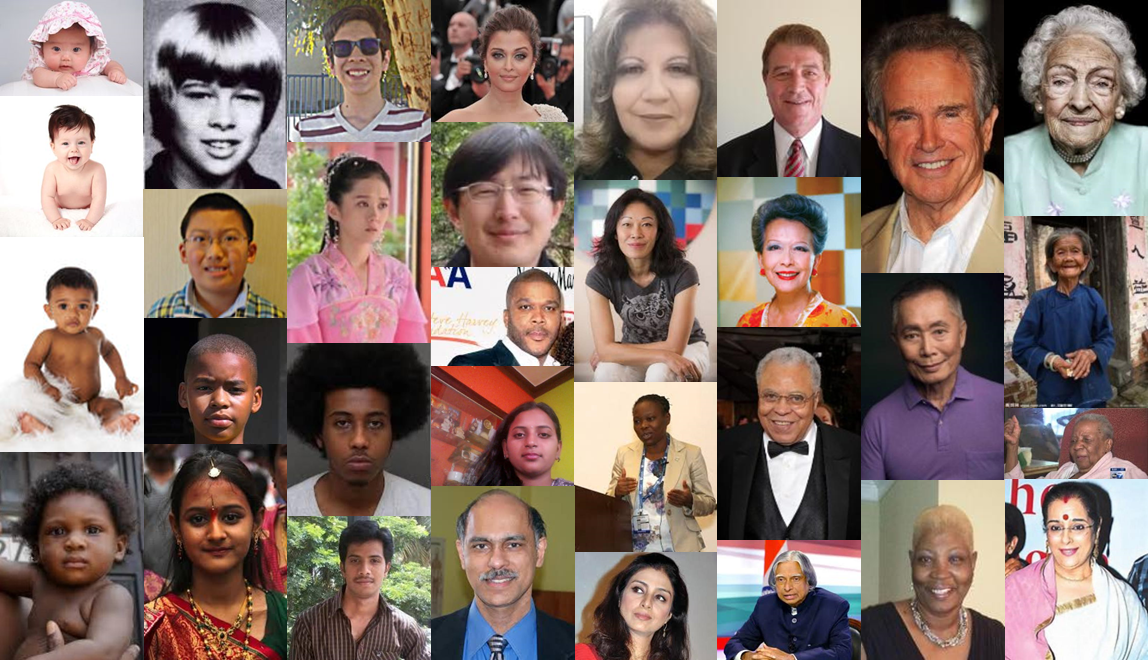
\includegraphics[scale=0.2]{gambar/UTKFace.png}
      % Label referensi dari gambar yang diinputkan
      \label{fig:UTKFace}
    \end{figure}

    \begin{center}
      % Keterangan gambar yang diinputkan
      Gambar 3.1 : Dataset UTKFace
    \end{center}

   \item [b.] Laptop \\
   Personal computer portable dengan spesifikasi prosesor intel i5 generasi lima, GPU nvidia Geforce 930M, 
   RAM 8GB dan storage 750GB akan digunakan untuk pembuatan model dan pencobaan model yang sudah jadi 
   menggunakan kamera yang tersedia pada perangkat.

   \item [c.] Google Collab \\
   Merupakan sebuah website yang dimiliki oleh Google yang dapat digunakan untuk membuat program dan 
   menjalankannya. Menyediakan beberapa pilihan untuk menjalankan program melalui koneksi internet dan 
   tidak membebani kerja komputer. Dalam tugas akhir ini berfungsi sebagai tempat menjalankan program 
   training dataset dan juga pembuatan model menggunakan GPU dalam cloud yang disediakan Google Collab.
\end{itemize}
   

\subsection{Metodologi Penelitian}
Metodologi yang digunakan dalam pengerjaan Tugas Akhir ini adalah sebagai berikut.
    % Contoh input gambar dengan format *.jpg
    \begin{figure} [H] \centering
      % Nama dari file gambar yang diinputkan
      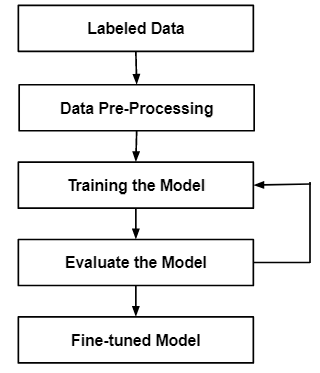
\includegraphics[scale=0.8]{gambar/Metodologi.png}
      % Label referensi dari gambar yang diinputkan
      \label{fig:Metodologi}
    \end{figure}

    \begin{center}
      % Keterangan gambar yang diinputkan
      Gambar 3.2 : Diagram blok metodologi
    \end{center}

\begin{enumerate}
   \item \textbf{Pemrosesan Dataset} \\
   Pada tahap ini dataset yang digunakan aakn dicek dan dibagi berdasarkan training, validation dan 
   testing, serta menyiapkan dataset untuk digunakan pada pembuatan model nantinya.
   \item \textbf{Pemilihan Model} \\
   Memilih model atau arsitektur Convolutional Neural Network atau CNN yang tepat sesuai dengan UTKFace 
   dataset yang telah disediakan sebelumnya dan membangun model untuk keperluan training.
   \item \textbf{Training} \\
   Pada tahap ini dataset akan digunakan untuk melatih komputer dengan cara mengolah gambar dan anotasi 
   yang telah dibuat sehingga terbentuk pola atau karakteristik dari masing masing kelas yang akan 
   menjadi bahan pertimbangan komputer dalam mencapai sebuah keputusan atau melakukan prediksi. 
   Proses training akan dilakukan menggunakan Covolutional Neural Network atau CNN pada citra wajah 
   yang diberikan.
   \item \textbf{Tuning} \\
   Model yang sudah jadi akan dievaluasi dan dilakukan pengaturan lagi untuk meningkatkan peforma dan 
   keakuratan model.
   \item \textbf{Pengujian dan Analisa} \\
   Sistem yang sudah jadi akan diuji pada dataset yang telah disiapkan untuk testing dan juga akan dicoba 
   pada kamera di wilayah ramai orang untuk mengumpulkan data. Kemudian data yang diperoleh dianalisa 
   dan dicatat untuk keperluan pembuatan laporan nantinya.
\end{enumerate}